\documentclass{beamer}

\usepackage{beamerthemesplit}
\usepackage{latexsym}
\usepackage{eurosym}
\usepackage[activeacute,spanish]{babel}
\usepackage{ae,aecompl}
\usepackage{graphicx}
\usepackage{amsfonts}

\usetheme{Darmstadt}

\title{Propuestas para Proyecto de Lenguaje de Programacion}
\author{G. Chavez - K. Campuzano - J. Camacho - K. Altamirano}
\date{22 de octubre de 2012}

\begin{document}

\frame{\titlepage}

\section[Indice]{}
\begin{frame}[allowframebreaks]
\tableofcontents
\end{frame}
%\frame{\tableofcontents}

\section{Propuesta 1}
\begin{frame}[allowframebreaks]
\frametitle{Cinem}
\begin{figure}[h]
\centering
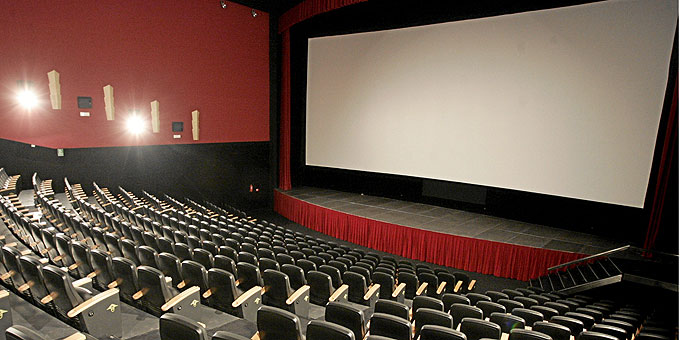
\includegraphics[height=0.5\textheight]{salacine.jpg}
\end{figure}
\end{frame}

\begin{frame}[allowframbreaks]
\frametitle{Cinem}
\begin{figure}[h]
\centering

\includegraphics[height=0.5\textheight]{apuro.jpg}
\end{figure}
\end{frame}

\begin{frame}[allowframbreaks]
\frametitle{Cinem}
\begin{figure}[h]
\centering
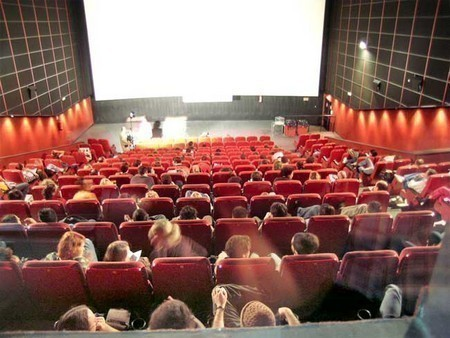
\includegraphics[height=0.5\textheight]{viendopelicula.jpg}
\end{figure}
\end{frame}

\begin{frame}[allowframbreaks]
\frametitle{Cinem}
\begin{figure}[h]
\centering

\includegraphics[height=0.5\textheight]{hambre.jpg}
\end{figure}
\end{frame}

\begin{frame}[allowframbreaks]
\frametitle{Cinem}
\begin{figure}[h]
\centering
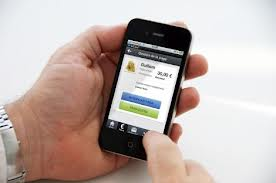
\includegraphics[height=0.5\textheight]{appenmovil.jpg}
\end{figure}
\end{frame}

\begin{frame}[allowframbreaks]
\frametitle{Cinem}
\begin{enumerate}
\item Numero de Asiento
\item Sala en la que se encuentra
\item Tiempo limitado para la compra (7min)
\item La compra se hara mediante tarjetas de debito de la misma sala de cine
\end{enumerate}
\end{frame}

\begin{frame}[allowframbreaks]
\frametitle{Cinem}
\begin{figure}[h]
\hfill
\begin{minipage}[t]{.45\textwidth}
\begin{center}
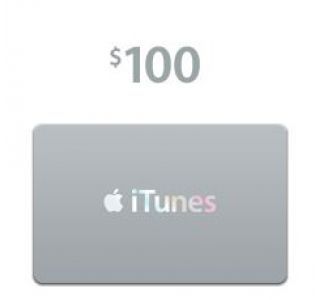
\includegraphics[height=0.5\textheight]{tarjetaapple.jpg} % primera imagen colocada a la izquierda
\end{center}
\end{minipage}
\hfill
\begin{minipage}[t]{.45\textwidth}
\begin{center}
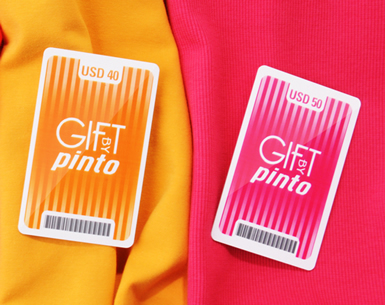
\includegraphics[height=0.4\textheight]{tarjetapinto.jpg} % segunda imagen colocada a la derecha 
\end{center}
\end{minipage}
\hfill
\caption{Tarjetas}
\end{figure}
\end{frame}

\begin{frame}[allowframbreaks]
\frametitle{Cinem}
\begin{figure}[h]
\centering

\includegraphics[height=0.5\textheight]{comida.jpg}
\end{figure}
\end{frame}


\section{Propuesta 2}
\begin{frame}[allowframebreaks]
\frametitle{Cuentas}
\begin{figure}[h]
\centering
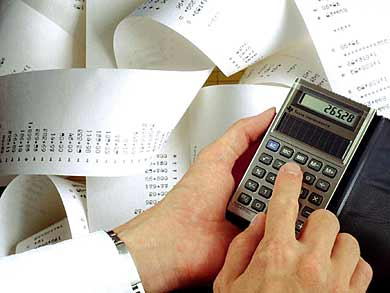
\includegraphics[height=0.5\textheight]{cuentas.jpg}
\end{figure}
\end{frame}

\begin{frame}[allowframbreaks]
\frametitle{Cuentas}
\begin{figure}[h]
\centering
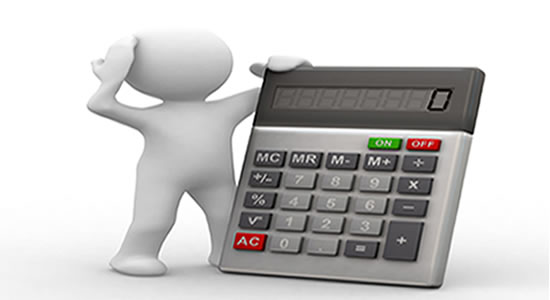
\includegraphics[height=0.5\textheight]{cuentas1.jpg}
\end{figure}
\end{frame}

\begin{frame}[allowframbreaks]
\frametitle{Cuentas}
\begin{figure}[h]
\centering

\includegraphics[height=0.5\textheight]{presupuesto2.jpeg}
\end{figure}
\end{frame}

\begin{frame}[allowframbreaks]
\frametitle{Cuentas}
\begin{figure}[h]
\centering
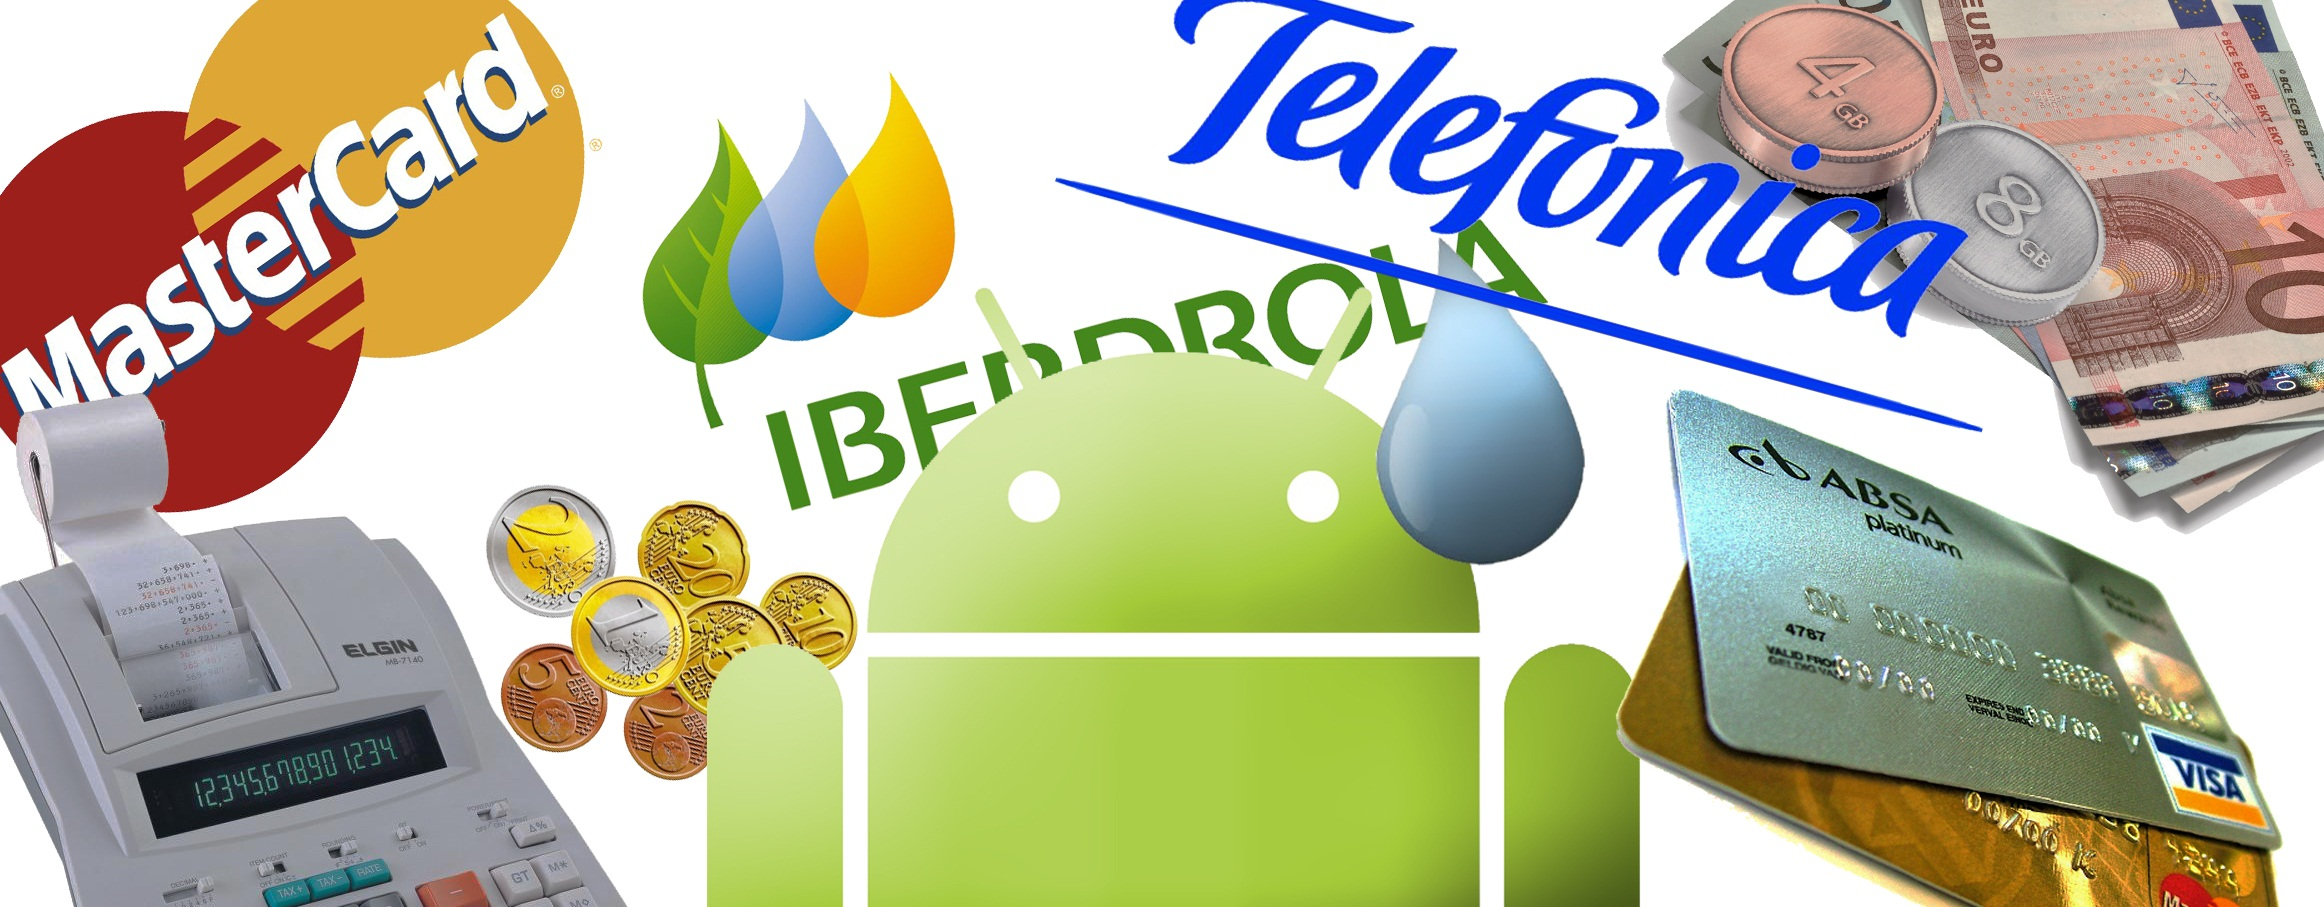
\includegraphics[height=0.5\textheight]{gastos.jpg}
\end{figure}
\end{frame}

\begin{frame}[allowframbreaks]
\frametitle{Cuentas}
\begin{figure}[h]
\centering
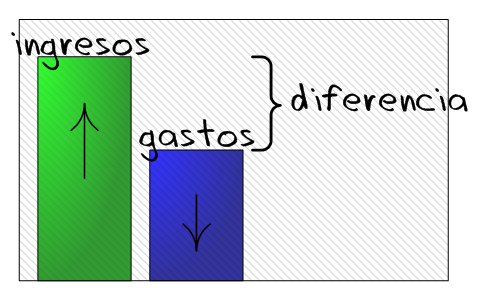
\includegraphics[height=0.5\textheight]{cuenta.png}
\end{figure}
\end{frame}

\begin{frame}[allowframbreaks]
\frametitle{Cuentas}
\begin{enumerate}
\item Controlar gastos diarios de una persona a partir de un saldo inicial
\item Registro cronologico de ingresos y gastos
\item Registro de ingresos y gastos en agrupaciones como alimentacion, transporte, etc.
\end{enumerate}
\end{frame}

\begin{frame}[allowframbreaks]
\frametitle{Cuentas}
\begin{figure}[h]
\centering

\includegraphics[height=0.5\textheight]{control.jpg}
\end{figure}
\end{frame}


\section{Propuesta 3}
\begin{frame}[allowframebreaks]
\frametitle{GasNext}
\begin{figure}[h]
\centering
\includegraphics[height=0.5\textheight]{Gasolinera}
\end{figure}
\end{frame}

\begin{frame}[allowframbreaks]
\frametitle{GasNext}
\begin{figure}[h]
\centering
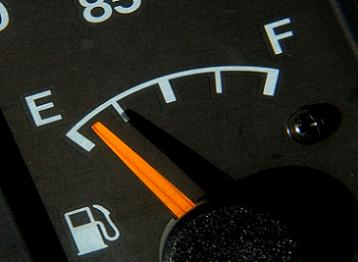
\includegraphics[height=0.5\textheight]{Casisingasolina}
\end{figure}
\end{frame}

\begin{frame}[allowframbreaks]
\frametitle{GasNext}
\begin{figure}[h]
\centering
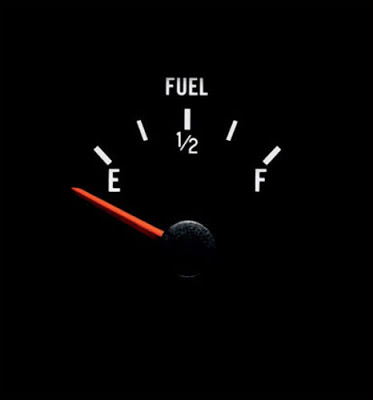
\includegraphics[height=0.5\textheight]{Sinnadadegasolina}
\end{figure}
\end{frame}

\begin{frame}[allowframbreaks]
\frametitle{GasNext}
\begin{figure}[h]
\centering

\includegraphics[height=0.5\textheight]{Dinerofull}
\end{figure}
\end{frame}

\begin{frame}[allowframbreaks]
\frametitle{GasNext}
\begin{figure}[h]
\centering
\includegraphics[height=0.5\textheight]{Dineroporelcaño}
\end{figure}
\end{frame}

\begin{frame}[allowframbreaks]
\frametitle{GasNext}
\begin{enumerate}
\item Guayaquil.
\item Indica las gasolineras m\'as cercanas.
\item Indica el precio de la gasolina en cada gasolinera.
\end{enumerate}
\end{frame}

\end{document}